\documentclass[12pt,a4paper,oneside]{book}
% Scheletro di sorgente LaTeX per la scrittura 
% di una tesi di laurea.
% Per la grafica 
%%UNUSED PACKAGES START
%\usepackage{forest}
%\usepackage{subcaption}
%\usepackage[]{mcode}
%\usepackage{tikz}
%\usetikzlibrary{matrix,chains,positioning,decorations.pathreplacing,arrows}
%\usetikzlibrary{arrows,automata}
%\usetikzlibrary{shapes,snakes}
%\usetikzlibrary{calc,arrows}
%\usetikzlibrary{scopes,matrix,positioning}
%\tikzset{%	
%  every neuron/.style={
%    circle,
%    draw,
%    minimum size=0.5cm
%  },
%  neuron missing/.style={
%    draw=none, 
%    scale=3,
%    text height=0.333cm,
%    execute at begin node=\color{black}$\vdots$
%  },
%x  neuron missingl/.style={
%    draw=none, 
%    scale=2,
%    text height=0.333cm,
%    execute at begin node=\color{black}$\vdots$
%  },
%}
%\usepackage{gensymb}
%% Per aggiungere la bibliografia nella \tableofcontents
%%\let\oldbib\bibliography
%\renewcommand{\bibliography}{\cleardoublepage1
%\addcontentsline{toc}{chapter}{\bibname}
%\oldbib}	
%\usepackage[nottoc]{tocbibind}
%\onehalfspacing

%\usepackage{epigraph}

%\usepackage[T1]{fontenc}

%\usepackage{microtype}
%\usepackage{enumitem} %personalizza liste puntate e numerate
%\setlist{leftmargin=*,nolistsep}
%\renewcommand\theenumi {\alph{enumi})}% lettere al posto di numeri
%\renewcommand\labelenumi{\theenumi}% parentesi al posto di punti
%\usepackage{eurosym}
%\usepackage[figure]{hypcap} %link nel pdf alla figura e non alla didascalia
%\linespread{1.5}
%%UNUSED PACKAGED END


\usepackage{graphicx}
\usepackage[a4paper,top=3.5cm,bottom=3cm,left=3cm,right=3cm,bindingoffset=5mm]{geometry}
\usepackage[utf8]{inputenc}

\usepackage{amsmath, amssymb, amsfonts}
\usepackage[pdfpagemode={UseOutlines},colorlinks=false,linktocpage=true,citecolor=blue,bookmarksnumbered=true,bookmarksopenlevel={3},pdfstartview={Fit},pdfpagelayout={SinglePage} ,hidelinks]{hyperref}
\usepackage[english]{babel}
\usepackage{array}
\usepackage{graphicx}
\usepackage{setspace}
\doublespacing
\usepackage{fancyhdr}
\usepackage{todonotes}
\usepackage{comment}

\setlength{\abovecaptionskip}{15pt plus 3pt minus 2pt}

%%abstract definition
\makeatletter
\if@titlepage
  \newenvironment{abstract}{%
      \titlepage
      \null\vfil
      \@beginparpenalty\@lowpenalty
      \begin{center}%
        \bfseries Abstract
        \@endparpenalty\@M
      \end{center}}%
     {\par\vfil\null\endtitlepage}
\else
  \newenvironment{•}{•}{•}newenvironment{abstract}{%
      \if@twocolumn
        \section*{Abstract}%
      \else
        \small
        \begin{center}%
          {\bfseries Abstract\vspace{-.5em}\vspace{\z@}}%
        \end{center}%
        \quotation
      \fi}
      {\if@twocolumn\else\endquotation\fi}
\fi
\makeatother
\usepackage{wrapfig}




%\bibliographystyle{IEEEtranN}



\begin{document}

\newgeometry{left=3cm,right=3cm,bottom=3cm,top=3cm}
\thispagestyle{empty}
\begin{center}

\includegraphics[height=5cm]{Figure/LOGO_UNISI.pdf}

\large{ \sc Dipartimento di ingegneria dell'informazione e scienze matematiche}
\vspace{0.5cm
\large Computer and Automation Engineering}\\
\vspace{0.5cm}
\large {\sc Robotics and Automation}
\vspace{1cm}
 
\vspace{\stretch{.8}}

%\textbf{\scshape{\LARGE{Handwritten classification of MNIST dataset\\with TensorFlow\\}}}
\textbf{\scshape{\LARGE{Handshake human-robot analysis\\}}}

\end{center}
\vspace{\stretch{1}}

\noindent\begin{minipage}[b]{0.47\textwidth}
%\begin{flushleft} 
\large
\emph{Professor:}\\
\textbf{D. Prattichizzo}  
%\emph{Correlatori:}\\
%\textbf{Dr. John Doe}
%\end{flushleft}
\end{minipage}
\hfill
\begin{minipage}[b]{0.47\textwidth}\raggedleft
 \large
\emph{Student:}\\
\textbf{Francesco Vigni}\\


\end{minipage}

%\begin{minipage}{0.5\textwidth}
%\begin{flushright} \large
%\emph{Tesi di laurea di:} \\
%\textbf{Francesco Vigni}
%\end{flushright}
%\end{minipage}
%
%\begin{minipage}[t]{0.47\textwidth}
%{\large{\bf Relatore:\\
%Prof. NOME RELATORE}}
%\vspace{5mm}\\
%{\large{\bf Correlatore:\\
%Prof. NOME CORRELATORE\\
%Prof. NOME CORRELATORE}}\\
%%\vspace{5mm}\\
%%{\large{\bf Relatore:\\
%%Chiar.mo Prof.\\
%%NOME CORRELATORE}}
%\end{minipage}
%\hfill
%
%\begin{minipage}[t]{0.47\textwidth}\raggedleft
%{\large{\bf Candidato:\\
%NOME LAUREANDO}}
%\end{minipage}


%\noindent RELATORI:\\
%Prof. Gigi Riva\\
%Prof. alskdj
%\begin{flushright}
%TESI DI LAUREA DI:\\
%kjsad aslkjd 

%\end{flushright}
%\vspace{\stretch{1}}
%\vfill
\begin{center}
\hrule
%\includegraphics[width=\columnwidth]{figure/skyline1}
\vspace{0.5cm}
\large{A.A. 2017-2018}
\end{center}
\restoregeometry



\tableofcontents
%\listoffigures
%\listoftables

% If you wish to include an abstract, uncomment the lines below
%Abstract text
%\abstract{

\begin{abstract}
%\textbf{Closed loop approach to Human-Robot Handshake}

\vspace{60px}
%----------------------------------------------------------------------------------------
%	SECTION 1
%----------------------------------------------------------------------------------------
%%\section{Environment}
The following work is focusing on the Human-Robot hand interaction, specifically in the grasping force of the handshake. The handshake event between human beings is a well known task, it can to enable a communication between participants as a mixture of physical features like: grip force of the hand, velocity approach, duration of the handshake, oscillation frequency and amplitude of the arm. The hypothesis is is that in human hand-shaking force control there is a balance between an intrinsic (open–loop) and extrinsic (closed–loop) contribution. The target of this work is to set up an environment in order to test the hypothesis for the human-robot handshake grip force.
The environment is built using Robotic Operating System (ROS), which is managing messages among: a Pisa/IIT SoftHand and three FSR 400 sensors managed by an Arduino Uno.
A detailed force analysis is needed in order to evaluate the grasping force in the human-robot handshake. The method is presented in \ref{subsec:calibFSR} is providing an estimation for the force the human applies on the robot $F_{h}$ and in \ref{ch:openloop} is presented a method for estimating the force the robot excerts on the human $F_{r}$.
The hypothesis is to model the human response to the robot grasp as a dynamical system.
A sensorimotor delay is mimicking the reaction time of Central Nervous System (CNS), and varying the contribution of intrinsic and extrinsic force control modify the perceived handshake quality in the user study. 
%
%%\\ 
% Abstract text
 \end{abstract}



%\chapter*{Introduction}
%The handshake event, commonly used, is a natural human interaction and is extensively used worldwide in events like: greetings, introduction routine between human beings and agreements. 
%The scientific approach to handshake between a human and a robot, therefore, must intrinsically deal with low levels human interactions and some assumption must be done in order to focus on the task.
%The handshake event can be divided in two parts: the approaching and the handshaking. This work is focused on the haptic sense involved during the handshake, knowing that the approaching is mainly executed using non haptic senses (f.i. vision).\\ %The full routine of the handshake event can be summarized in a starting time, a duration. Assuming the human to be in a leading position both, the starting point and the duration of the handshake are decided by the human.
%An interesting parameter involved in the handshake is the consensus; it allow the human to evaluate a handshake mixing aspects like: duration of the event, dynamics, force exchanged.
%An important part of this work is to test different controllers with the purpose of evaluating the consensus using closed loop controllers. 
%  
%Many research teams all over the world are focused on the human-robot physical interaction, this opens the topic to an interesting scientific discussion.  
\chapter*{Introduction}
Developing a robot capable of performing a smooth human-like handshake is becoming a highly interested topic in the scientific literature.
A natural handshake between two humans is a very complex task to replicate, this work just focuses on the interaction force between a robot hand and a human hand.
In many parts of the world, the handshake is an important interaction task both for business and social context \cite{chaplin2000handshaking}, and an important behaviour to identify is the consensus in the event. It is reasonable to assume that in human-human handshake consensus is reached using not just the haptic sense for the task. Due to the nature of this behaviour it is complex to embed inside a robot, participants will easily distinguish the event with respect to another human or to a robot. It is assumed that humans will naturally take into account for evaluating a handshake not just the grip force but also the skin feedbacks, vision and prior expectations. However, there is little work in the literature studying human-human handshaking, and as such it is not yet possible to describe what constitutes a ‘good’ or a ‘bad’ handshake, or even describe a human-human handshake, in a quantitative manner.
In Human Robot Interaction \cite{sheridan2016human}, the handshake is a really interesting task to focus on, typically leader and follower roles are clearly defined, master action is measured and elaborated to generate reference inputs for the slave controller. In handshake this prior allocation of roles is not defined, it is an inherently bidirectional action in which both sides actively contribute to the task by applying an active and a reactive action at the same time.
%


Authors in \cite{pedemonte2016design}  present the design and realisation of a haptic interface performing a robotic handshake, the device is aimed at developing a communication system that allows two people to shake hands while being in different locations. 

Another device for the realisation of realistic human-robot handshake is presented in \cite{arns2017design}, in particular in this work a standard characteristic model of the human-palm compliance is developed, based on human hand anatomy and an empirical study.
	
The goal of these systems is to appear as a transparent haptic link between the two participants, so that the dynamics of their interaction is similar to in a direct physical handshake. This is different to the goal of this work, which is to realise a robotic autonomous setup able to emulate the human dynamics in handshaking tests.
%
A study in human-robot handshaking \cite{Tsalamlal2015}, investigates the effect on perceived affective properties as the arm stiffness, grasping force and robot facial expressions are changed. 
%
A handshake can be considered to include multiple phases. In the approach phase, both partners rely on vision in order to establish contact. Next, in the handshaking phase, each partner exerts a force by closing the hand and receives a force from the other partner. 
For the case of a human-robot handshake, the robot will receive a force from the human $F_{h}$, and also exert a force $F_{r}$ on the human. Finally, the handshake is concluded by one partner releasing the grasp and the second partner following.
%	
A haptic virtual reality system which allows human to make physical handshakes with a virtual partner is presented in \cite{wang2011handshake}. Two approaches are proposed: in the first one robot controller employs an embedded curve and disregards human interaction, in the second one an interactive control is implemented; they verified that the second one is perceived more human-like. 
In \cite{karniel2010turing} is proposes a Turing-like handshake test to compare a human-human handshake, realised through a haptic interface, with different virtual handshake models.
Both \cite{wang2011handshake} and  \cite{karniel2010turing} focus on arm trajectory and disregard handshake force. 
For grasping and manipulation tasks, there is a substantial number of studies looking at how the grip force is modulated \cite{johansson1992sensory,eliasson1995development,witney2004cutaneous}, these works show that cutaneous feedback is also used to avoid slip. 
%
This principle has also been applied to robotic grasping: authors in \cite{ajoudani2016reflex} propose a system for modulating the grasp strength in a reflexive manner to avoid object slippage.\\
%
%This is different to a handshaking interaction, and it is therefore not clear to what extent these dynamics will also be applicable for a handshake.

%These are some characteristics that are still not embedded into the hardware available in the market.
%The grasping force exchanged in the human-robot handshake event is a complex value to identify, this work is estimating the grasping force from values which can be clearly identified. 


%The aspect taken in consideration in this work is the grasping force exchanged in the handshake therefore, an accurate choice has been done on the hardware to use in this work.
The robot hand chosen for this work (Pisa/IIT SoftHand \cite{catalano2014adaptive) had been instrumented with force sensitive resistors in a position where \cite{knoop2017handshakiness} shown important contact pressure distribution.
Although force sensitive resistors are really useful in this work thanks to their width, a calibration method is needed in order to obtain an estimation of the human grasping force. %The calibration exploit the idea in \cite{calibFSR}, by comparing force sensitive resistor measurement with a load cell.
Position reference of Pisa/IIT SoftHand can be controlled, but for a more consistent analysis a measure of robot grasping force is needed. 
\include{chapters/idea}
\include{chapters/hardware}
\include{chapters/software}
\include{chapters/openloopexp}
\include{chapters/proposedcontrollers}

\include{chapters/results}
\include{chapters/conclusion}

%\chapter{The state of the Art}
Develop a robot capable of performing a smooth human-like handshake is still a highly interested topic in the scientific literature.
A natural handshake between two humans is a very complex task to replicate, this work just focuses on the interaction force between an artificial hand and a human hand.
The consensus is a complex task to encode inside a robot, participants will easily distinguish the event with respect to another human or to a robot. A human will take into consideration the skin feedbacks like: the temperature, the humidity and the softness. These are some characteristics that are still not embedded into the hardware available in the market. The aspect taken in consideration in this work is the grasping force exchanged in the handshake. 
Robots, nowadays, are highly involved in industries where mostly they have to execute repetitive tasks. These kind of robots, when have to grasp objects, commonly uses multi purposes grippers \cite{multipurposegripper}, therefore, an accurate choice has been done on the hardware to use in this work. 
%The grasping force exchanged in the human-robot handshake event is a complex value to identify, this work is estimating the grasping force from values which can be clearly identified. 


\cite{facialexpressions}
\cite{mirrorgame}
\cite{papageorgiou}

\section{The Idea}
The idea is to create a closed loop controller for the human-robot handshake event, using Pisa/IIT SoftHand produced for research purposes at Universit\`a degli studi di Pisa and Istituto Italiano di Tecnologia (IIT) and upgrading it with four independent FSR sensors which uses an Arduino uno in order to communicate the data.
The FSR sensors are located on the robotic hand so there are no wearing device on the human hand during the execution of the experiments.
This choice leads the work to be focused on the theoretical part of the handshake event, and potentially reach robust results. We are focusing on a general human-robot handshake, knowing that the interaction can vary with participants, f.i. the participant's hand size is affecting the firsts contact points or nominal strength to apply in the handshake can be affected by prior expectations. It is more meaningful then, to study individual differences once the generic case has been studied.
The chosen robotic hand (Pisa/IIT SoftHand) has 19 degrees of freedom and its main characteristic a single dc motor that is pulling a tendon which is embedded in each finger. This physical approach results in an under actuated robotic hand which can be controlled only by the dc motor and can easily adapt to different configurations without modifying the reference position. 

\chapter{Hardware setup}
The hardware must be physically merged in order to reach the goal of a closed loop controller for a handshake. From early approaches as \cite{espen}, an estimation of the human palm has been used.  The \textit{sensorized palm} idea was to approximate the human palm which is the part of the hand mostly interested during a handshake.
The figure \ref{fig:sensorsONhand} shows the position in which the sensors are placed, both sensors n. 1, 2, 3 are placed according studies in \cite{espen}. \\ \\
%, the sensor n. 4 is placed in order to increase the weight of human-thumb force applied during the grasp.\\ \\

\begin{figure}[h]
  \centering
  \begin{minipage}[b]{0.4\textwidth}
    \includegraphics[width=\textwidth]{Figure/qbhand1.png}
    
  \end{minipage}
  \hfill
  \begin{minipage}[b]{0.4\textwidth}
    \includegraphics[width=\textwidth]{Figure/qbhand2.png}
  \end{minipage}
  \label{fig:sensorsONhand}
  \caption{Pisa/IIT SoftHand with FSR sensors for handshake}
\end{figure}

\section{The Pisa/IIT SoftHand}\label{sec:softhand}
The Pisa/IIT SoftHand is a simple, robust and effective hand designed for grasping and soft manipulation presented in \cite{catalanopisa}. A tick range is provided with the device in order to set a range of possible closure positions, more formally, let's define $q \in \mathbb{N}$ as the closure position of the hand such that $max(q) = 19000$ (Pisa/IIT SoftHand fully closed) and $min(q)=0$ (Pisa/IIT SoftHand fully opened). The hardware is provided with a controller developed by the same group which implements a proportional controller Fig. \ref{Fig:Pr} on the motor position. This enables the researchers to control the Pisa/IIT SoftHand with a reference position, without dealing with the current control of the motor. \\
\begin{figure}[h]
\centering
\includegraphics[width=0.6\textwidth]{Figure/softhand.png}
\caption{Exploited view of the modules of Pisa/IIT SoftHand}
\label{Fig:Softhand}
\end{figure}
The proportional coefficient can be set up as preferred since its encoded in ROS as a \textit{rosparam}, this parameter is thought to range between 0 and 1.0. Setting the parameter to 1.0 is minimizing the error value $e(t)$  between the setpoint $r(t)$ and the output $y(t)$.
The successful idea in the design of Pisa/IIT SoftHand can be found in the flexibility of the joints and the wide range of usage.
The reference position $r(t)$ has no 1:1 correspondence with the single physical position of each finger. Having a single motor to control makes the robotic hand really easy to control but introduce uncertainty on the position of each finger. 
A tendon is running through all the fingers and is pulled by the internal dc motor, therefore a useful available information is the overall tick-position of the Pisa/IIT SoftHand. Constraints on the closure position $q$ are defined as follows:

\begin{equation}
q \in \mathbb{N} : \left\{\begin{matrix}
max(q) = 19000 \\ 
min(q) = 0
\end{matrix}\right.
\label{EQ:qlimits}
\end{equation}

The device has an internal value returning to the system the real tick position, this value is compared with the referenced one in the controller. The real tick position is a value that must be calibrated manually using administrative tools provided by the manufacturers. 
The calibration is manual which means that the Pisa/IIT SoftHand is manipulated to be into a fully open position and the program save that position as the zero tick position.
%The controller used $C(s)$ is a simple constant controller with value ranges from 0 to 1. 

\begin{figure}[h]
\centering
\includegraphics[width=0.5\textwidth]{Figure/feedbackP.png}
\caption{Block Diagram Proportional controller in a feedback loop}
\label{Fig:Pr}
\end{figure}


\section{The Sensors}
The core of the closed loop control is to have a feedback in the whole system which is proportional to the force applied during the handshake from the human. 
\begin{wrapfigure}{R}{0.3\textwidth}
\centering
\includegraphics[width=0.25\textwidth]{Figure/fsrsingle1.png}
\caption{FSR 13mm}
\label{Fig:FSRsingle}
\end{wrapfigure}

The sensors used in this work are Force Sensitive Resistors Fig. \ref{Fig:FSRsingle} measuring the force applied from the human to the Pisa/IIT SoftHand, in order to decouple this force from the one applied from the Pisa/IIT SoftHand to the human hand, \cite{espen} has been used and the physical position of the FSRs has been setted up accordingly.
FSR sensors are devices that allow to measure static and/or dynamic forces applied on the sensing area, through the variation of its electric resistance. The main advantage of these devices is the low cost per-unit, little space required for installation (thickness under 1.25mm) and the force sensitivity range up to 20N.\\
As robust polymer thick film devices, the FSRs, exhibit a decrease in electric resistance with increase in force applied to the surface. By theory is considered that when a force is applied the resistance changes approximately linear in a logarithmic plot \cite{fsrdatasheet}.
A simple force to voltage conversion is physically implemented as suggested the manifacturer, in fig. \ref{Fig:FSRcircuit} is shown a snippet of the above cited data sheet. For this work \textit{RM} is fixed to $3.3 k \Omega $. \\
\begin{figure}[ht]
\centering
\includegraphics[width=0.8\textwidth]{Figure/fsr.png}
\caption{FSR Datasheet snippet}
\label{Fig:FSRcircuit}
\end{figure}
These mentioned sensors are the more natural choice for handshake experiments since their thickness keeps the size of the Pisa/IIT SoftHand reasonable for human-robot handshake.
% 
Ideally using more sensors allow to get more relevant data but the surface available on the Pisa/IIT SoftHand is limited. The choice in the number of FSR sensors comes from the trade off between using lots of FSR sensors but with a smaller area and using a smaller amount of sensors but with higher area. The first configuration does not ensure the contact among experiments with different participants and the second configuration leads to physical bending of the sensors and influences the consistency of the readings.

 %A calibration method must be used in order to have robust results.

\subsection{Calibration of FSRs}
The calibration procedure of a sensor is a really important task, since it allow to compare experiments and to provide consistent results. 
The first voltage-to-force relation for the FSRs comes from a manufacturer sketch which is returning force with measures standard of grams.
As shown in \cite{calibFSR}, load cells can be used as 'ground truth' to calibrate force sensitive resistors to provide informations in Newtons. 
Using a \textit{sensorized palm} developed in \cite{espen}, sketched in Fig. \ref{fig:dummi} which embeds a load cell and placing the FSR sensors accordingly with the position of the sensors on the Pisa/IIT SoftHand; values from FSRs and the load cell are compared.\\
Mathematical regression tools have been used in order to find a model that explain the values from the sensors compared to the force of the load cell.
Although an exact calibration of FSR sensors is not the target of this work, a model has been fitted to the data in the force-range of interest of this work.
%The number of FSR sensors involved in the calibration experiment is two, instead the amount of FSR sensors chosen for the human-robot handshake is four. 
The configuration for the calibration experiment, with the \textit{sensorized palm} and two FRS sensors is shown in Fig. \ref{fig:dummifsr}. 
The position of the FSR sensors has been chosen accordingly to the position of the FSR sensors N.1 and N.2 on the Device \ref{fig:sensorsONhand}.
%In order not to add complexity to this task, is assumed that using two FSR are sufficient to fit a model to the FSR sensors involved in the handshake environment.
The experiment consist in apply a grasp to the device including not exclusively, the FSR sensors in the grasp. In post processing a model is fitted to the data and eventually allow the FSR to correcly estimate the grasping force.

\begin{figure}[h]
  \centering
  \begin{minipage}[b]{0.4\textwidth}
    \includegraphics[width=\textwidth]{Figure/dummipalm.png}
    \caption{Sensorized palm}
  \label{fig:dummi}
  \end{minipage}
  \hfill
  \begin{minipage}[b]{0.4\textwidth}
    \includegraphics[width=\textwidth]{Figure/dummipalmside.png}
    \caption{Sensorized palm with FSRs}
    \label{fig:dummifsr}
  \end{minipage}
  %\caption{FSR sensors position on sensorized palm}
\end{figure}



The experiment is executed with a participant applying different forces on the above mentioned device, and recording the output from the FSR sensors and from the load cell of the \textit{sensorized palm}.
The plot in Fig. \ref{Fig:FSRcalibratedModel}, shows the data obtain from this experiment.
Taking $N=2$ as the number of FSR sensors installed on the Pisa/IIT SoftHand, $F_{fsr,i}$ as the measure of the generic $i-th$ sensor, \textcolor{magenta}{the non calibrated grasping force is estimated as} %\ref{EQ:sumofFSR}.

\begin{equation}
\hat{F}_{fsr} = \sum_{i=1}^{N} F_{fsr,i}
\label{EQ:sumofFSR}
\end{equation}

A toolbox for data fitting from Matlab has been used in order to find the best fitting equation, that includes the origin, according to the Least Mean Square Error to the raw data, which analytically is:

\begin{equation}
F_{fsr} = 2.863 \cdot 10^{-9}\cdot \hat{F}_{fsr}^3 - 1.851 \cdot 10^{-5} \cdot \hat{F}_{fsr}^2 + 0.04863 \cdot \hat{F}_{fsr} 
\label{EQ:fsrdummyfit}
\end{equation}
where $\hat{F}_{fsr}$ is the value taken as the sum of the FSRs sensors, in this experiment two FSRs has been used.
The variable $F_{fsr}$ is returning Newtons and best explain the FSRs values with respect to the values of the \textit{sensorized palm}.

 
\begin{figure}[h]
\centering
\includegraphics[width=0.7\textwidth]{Figure/fsrtodummy.png}
\caption{FSRs vs. Load Cell data}
\label{Fig:FSRcalibratedModel}
\end{figure}

Obviously, more advanced models can be fitted in order to have FSR sensors returning Newtons with a higher precision, but for the specific task required in this work is considered sufficient the fitted equation in \ref{EQ:StepSignal}. The handshake event is involving grasping forces in a limited range of forces, the fitted equation exists for $ \hat{F}_{fsr} \in \mathbb{R}$, physical limitation of the hardware (max absorbed current) are ensuring the upper bound of the force. Till this point nothing has been done on the Pisa/IIT SoftHand, the available information is that FSR sensors are returning values in Newton and has been calibrated according to a load cell sensor, therefore forces in the following chapters will be intended to be Newton scaled. 
%The data collected in this experiment contains several outliers from the fitted equation, this behaviour is due to the 

\chapter{Software setup}
The described experiments can be implemented using a software capable of exchanging informations between robots, without the interaction of a human. A tool named Robot Operative System has been chosen in order to manage the informations between the devices involved in these experiments.  
\section{Ros}
The Robot Operative System (ROS) is a set of frameworks and libraries useful for robot software development. The logic of this software is really intuitive, it lets the developers to represent a device as node inside a graph. The most important node is this graph is the \textit{Master}, which is managing all the messages in the system. Each node in order to send or receive messages to/from other nodes must communicate this intention to the \textit{Master} node, which is processing the request and forwarding the right informations.\\
The result is a graph is built as a network of ROS nodes.
The main concepts in the ROS graph are ROS Nodes, Master, Parameter server, Messages,
Topics, Services, and Bags. 
%Each concept in the graph is contributed to this graphin different ways.
Each message in ROS is transported using named buses called topics. When a node sends a message through a topic, then it can be asserted that the node is publishing a topic. When a node receives a message through a topic,
then we can say that the node is subscribing to a topic but the production of information and consumption of it are decoupled. Each topic has a unique name, and any node can access this topic and send data through it as long as they have the right message type. The type of a message can be chosen among the standard primitive types (integer, floating point, Boolean, and so on) or custom message types can be defined. Custom field structure of messages are useful in order to send multiple message type over the same channel (topic).
%The ROS graph is oriented since the messages between nodes are edges of the graph passing the information from the node who is publishing to the one subscribed to it.

\section{Nodes}
The main aim of ROS nodes is to build simple processes, this makes debug easier and simplify the structure of a project. Each ROS node is written using ROS client libraries such as roscpp and rospy, in short a ROS node can be written as a C++ source file or as a python executable program. 

\subsection{Pisa/IIT SoftHand node}
Pisa/ITT SoftHand is provided with a variety of ROS packages, in particular, ROS node \textit{qb\textunderscore force\textunderscore interface} is the node managing the proportional controller on the position of the Pisa/IIT SoftHand. This node is publishing a topic named: /qb\textunderscore class/hand\textunderscore measurement which embeds a custom field structure named: qb\textunderscore interface/handPos. This custom type message embeds inside a package three float values with the meaning respectively of: sensed current position $q_{output}$, absorbed current, error between $q_{output}$ and $q_{ref}$.

\subsection{FSRs node}
The FSRs are connected to a bare PCB, each one following the circuit diagram in Fig. \ref{Fig:FSRcircuit}; This allows the source code flashed on the Arduino to: read the voltage difference at FSRs terminals, publish the information to ROS.
% apply the linear model for force measurements and publish the information to ROS.
A specific protocol called \textit{rosserial} is used in order to implement a ROS node with Arduino Uno.

\subsection{Auxiliary nodes}
The hardware related nodes of the project are now up and running, but in order to manage the informations and to eventually save files during the execution of the experiments, auxiliary nodes are created.
The auxiliary nodes are written in C++ or Python and the choice is strictly related to the compatibility with specific library (f.i. \textit{SMACH} State MACHine is a library used to implement state machines, currently only available in Python).
Several auxiliary nodes have been created in order to manage:

\begin{enumerate}
\item FSR calibration experiments
\item Saving data during experiments
\item Open loop experiments
\item Closed loop experiments
\end{enumerate}
Again, ROS provide the concept of node which is extremely useful for splitting work in smaller and more manageable units.

\chapter{Open Loop Experiments}
The open loop experiments aim to verify the hypothesis that the human response to a robot handshake can be modelled as a dynamical model. In these experiments human participants are intended to be a natural calibration system for the robot grasping force $F_r$. The hypothesis on participant's grasping force is shown in \ref{EQ:forceSteady}, participants are asked to apply the force that they are perceiving during the experiments.
\begin{equation}
F_{h} = F_{r}
\label{EQ:forceSteady}
\end{equation}
this introduces a limitation on the evaluation of the data, in fact the equation is assumed to hold only in quasi-static systems. A procedure to filter the transient from the data is applied in order to evaluate the relation $q$ vs. $F_h$ when steady states are reached.
Force is exchanged during a handshake only after the reference position has reach the first contact point $q_0$, therefore for values of $q < q_0$ no force will be exchanged in the handshake. The constraints on $q$ introduced in \ref{sec:softhand} are valid through all this work since are hardware related.
The \textit{sensorized palm} is used in order to seek the force behaviour for values of the reference position $q > q_0$. The shells of the device are not deformable, due to the material used during the 3D printing. Increasing the reference position $q$ of the Pisa/IIT SoftHand squeezing the \textit{sensorized palm} showed a linear relationship between the difference $q-q_0$ and $F_r$, as	 
%\textcolor{magenta}{talk about why the spring relation is choosed}

\begin{equation}
F_{r}(q)=\left\{\begin{matrix}
k_{r}(q-q_0) & $ for $ &q-q_0 \geq 0 \\ 
0 & $ for $ & q-q_0 < 0
\end{matrix}\right.
\label{EQ:genericForce}
\end{equation}

%
%$$
%F_{r} = 
%  \begin{cases} 
%    $Dynamic to find$ & q-q_0 \geq 0 \\
%    0 & q-q_{0} < 0
%  \end{cases}
%$$\\

Where $F_r$ is the force during the handshake applied by the robot on the \textit{sensorized palm}, $q$ is the reference position sent to the device.
During these experiments each reference position of the Pisa/IIT SoftHand is held for 3 seconds, the frequency rate of is set to 100Hz. \\
A file standard has been created in order to compare different experiments. The file is a '.csv' file with columns [FSR1, FSR2, Current, Real Position, Reference Position]. All the plots below are obtained as processing files with the previous structure. Each experiment starts with reference position set to 0 and finish with the reference position set to 0. \\
\section{Safety}\label{sec:safety}
The experiments are in open loop so in order to avoid injuries an emergency function has been created, if the participant starts feeling pain the key '\textbf{x}' on the keyboard must be pressed. The Pisa/IIT SoftHand will take as reference position 0 (fully open) and the whole program will be stopped.
In case of emergency the file will be saved and the last data can be used to understand the configuration just before the trigger event.\\
The experiments are done with the Pisa/IIT SoftHand in a horizontal position (palm facing down) Fig. \ref{Fig:palmdown}. In this way the weight of the Pisa/IIT SoftHand will not affect the FSR readings. 

\begin{figure}[ht]
\centering
\includegraphics[width=0.6\textwidth]{Figure/stand.png}
\caption{Palm facing down environment}
\label{Fig:palmdown}
\end{figure}

\section*{Participants}\label{sec:participants}
The participants to the experiments have been selected in an heterogeneous fashion from male to female with ages in (24-35 years old). Although the hand sizes available for the experiments are considered sufficient, over bounding the ranges of the previous age set can provide interesting results.
This experimental part is looking for the existing of the relation above mentioned \ref{EQ:genericForce}, therefore it is providing the methodology approach to this problem.
Each participant is repeating each experiment five times, this provide useful information and allow to average the outcomes of the same participant.

\newpage
\section{Step input}
The simplest signal that can be sent to the Pisa/IIT SoftHand is a step signal on the reference position, in this way the participant's response can be evaluated. The step signal in this experiment is formally a shifted and scaled step signal, the transformation parameters has been chosen in order to start from a position without physical contact to a position where empirical experiments have shown a consistent contact. 
%The first three seconds of the experiment $q_0$ is sent, then $q_1$ is sent so that the whole experiment lasts 6 seconds.
\begin{equation}
Q_{r}(t)=\left\{\begin{matrix}
q_{0} & $ for $ & t < t_0 \\ 
q_{1} & $ for $ & t \geq t_0
\end{matrix}\right.
\label{EQ:StepSignal}
\end{equation}
%$$
%Q_r(t) =   
%\begin{cases} 
%k_0 & t < t_0\\
%k_1 & t \geq t_0
%\end{cases}
%$$
%with $k \in \mathbb{R}$.
\subsection{Description}
The parameters chosen for the experiment in order to go from a reference position where $F_h=0$ to a reference position where $F_h > 0$ are:
\begin{itemize}
\item $q_0 = 8000 $
\item $q_1 = 15000$
\item $t_0 = 3s$
\end{itemize}
the experiment lasts in total 6 seconds. A correlation between the reference position of the Pisa/IIT SoftHand and the values recorded from the FSRs is expected. The participants are applying a force ($F_{h}$) which is assumed to be proportional to the one applied from the robot to their hand during the handshake \ref{EQ:forceSteady}.
The same experiment has been executed with multiple participants, in order to increase the amount of data available for the model estimation. The values of reference position in this experiment $q_{0}$ and $q_{1}$, are fixed during multiple trials, therefore the participants are able to predict that at $t=t_0$ a higher reference signal is sent. Although, this behaviour has been considered not consistent to fit, in post processing, a model to the data, it can provide a first sight the relation $q$ vs. $F_h$.
%
%\textcolor{magenta}{insert unfiltered plot of q vs force}
%
%\begin{figure}[h]
%  \centering
%  \begin{minipage}[b]{0.4\textwidth}
%    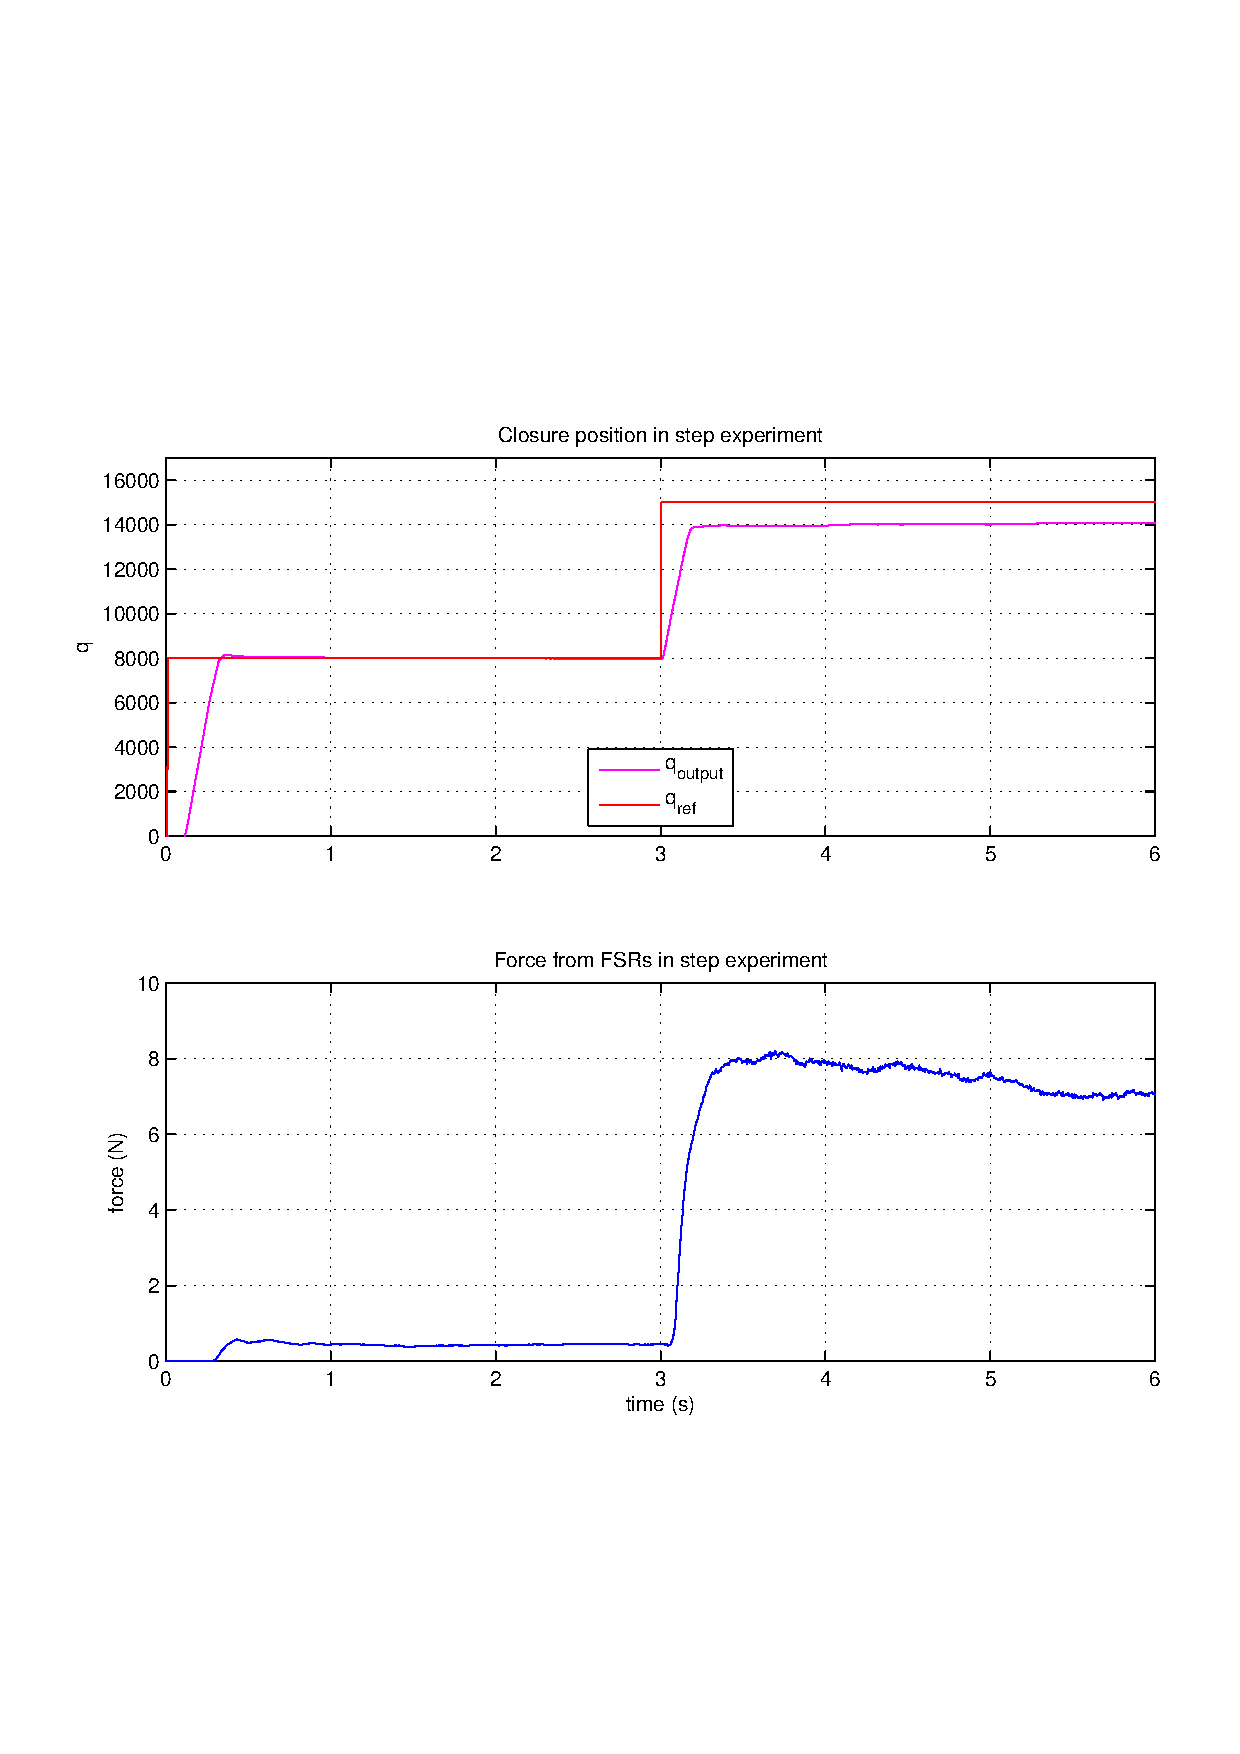
\includegraphics[width=\textwidth]{Figure/step.png}
%    \caption{Step experiment without transient}
%  \label{fig:step}
%  \end{minipage}
%  \hfill
%  \begin{minipage}[b]{0.4\textwidth}
%    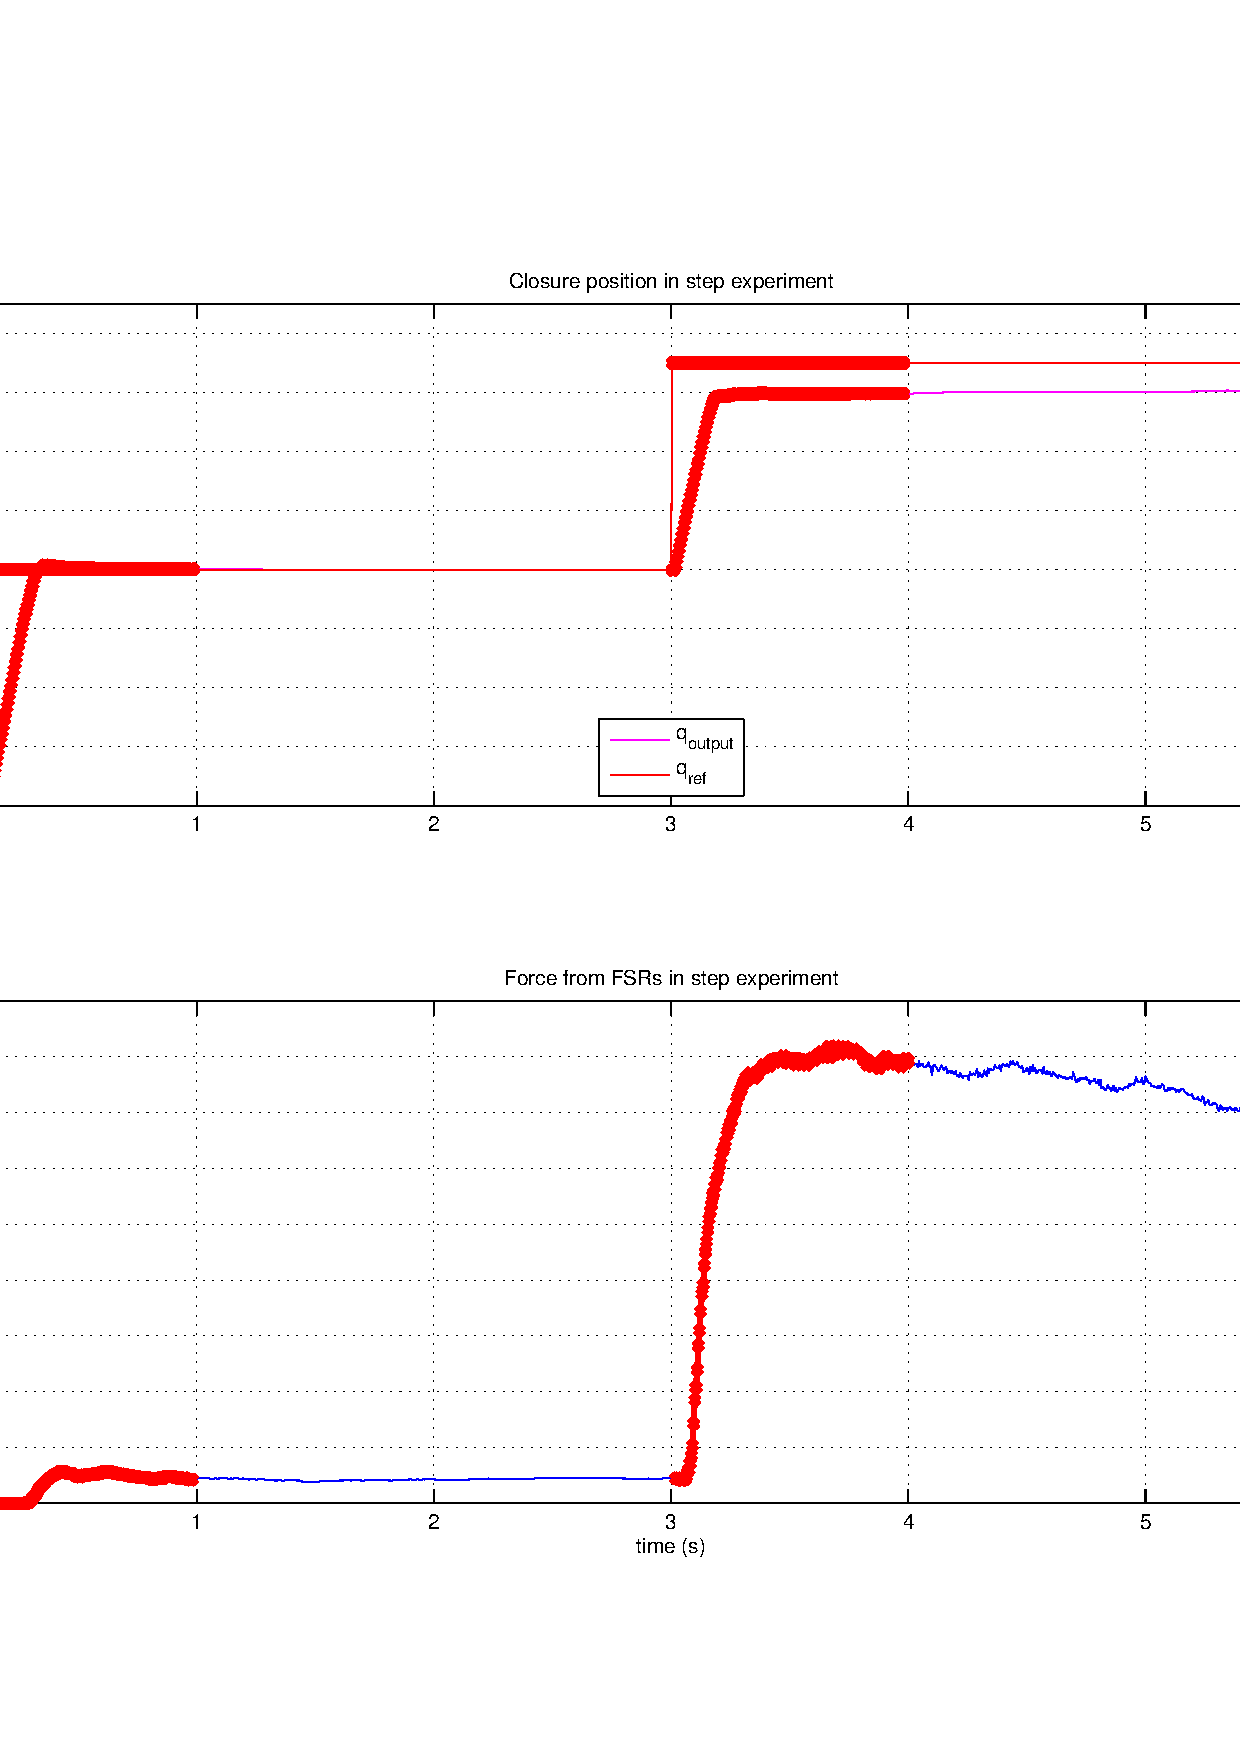
\includegraphics[width=\textwidth]{Figure/steptransient.png}
%    \caption{Step experiment with transient}
%    \label{Fig:steptransient}
%  \end{minipage}
%  %\caption{FSR sensors position on sensorized palm}
%\end{figure}
\begin{figure}[h]
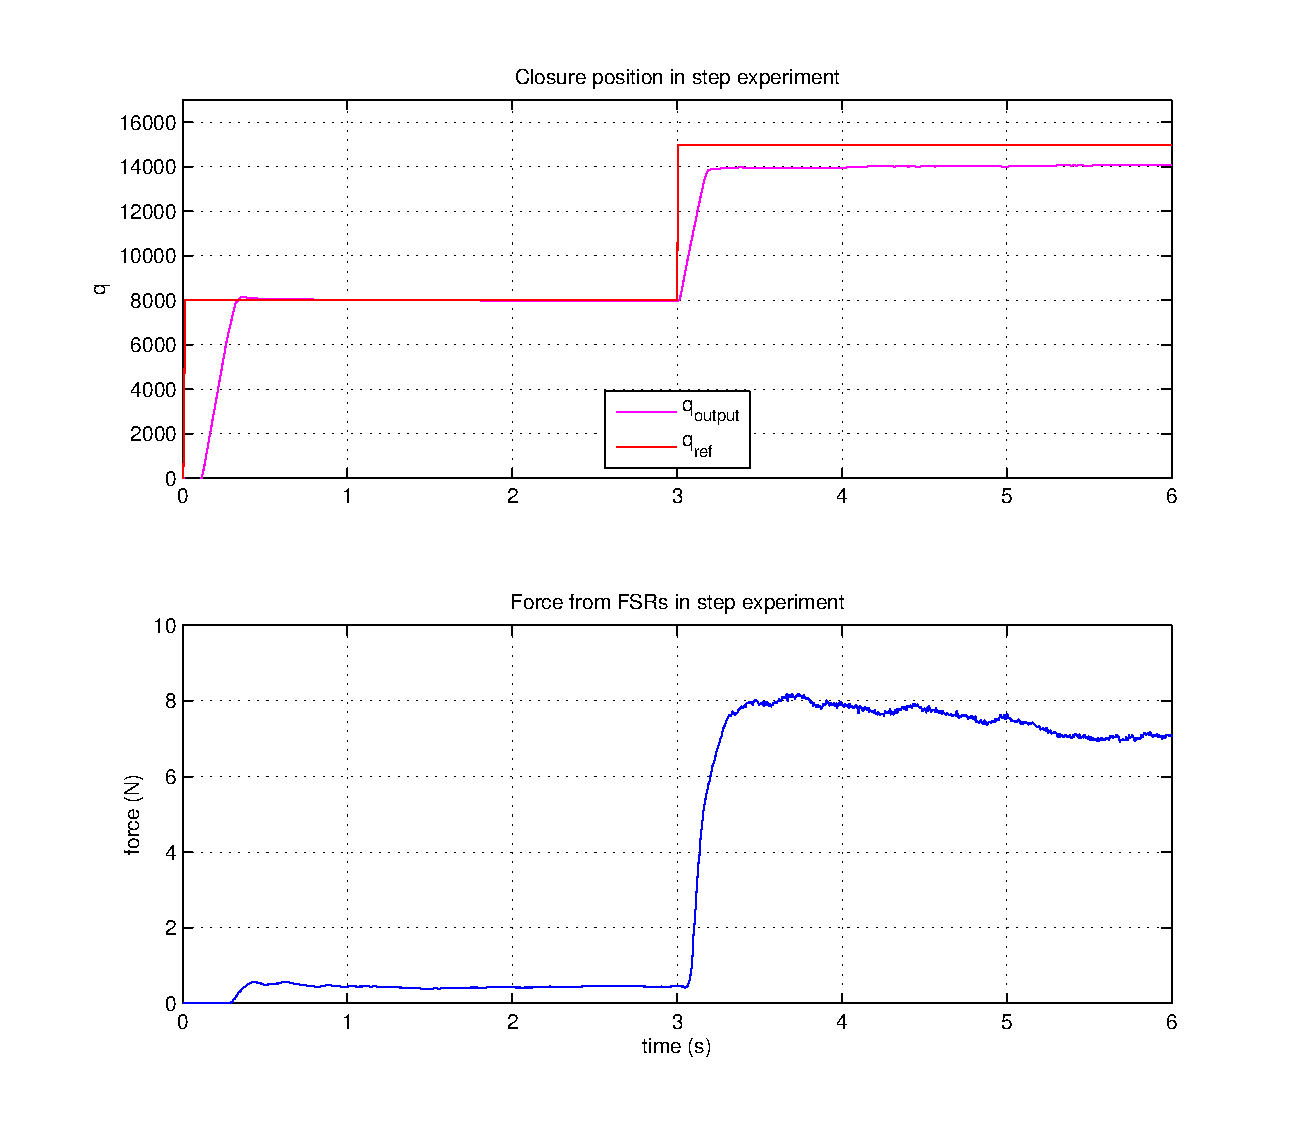
\includegraphics[width=\textwidth]{Figure/step.eps}
  \caption{Step experiment in time}
  \label{Fig:step}
\end{figure}

\textcolor{magenta}{insert step experiment plots force vs q}
\subsection{Transient filter}\label{sec:transient}
Giving as input to the system only two different values of reference position, makes more challenging to estimate a realistic model but it can already suggest that a correlation between $F_{h}$ and $q$ exists.
The Fig. \ref{Fig:step} shows the trend over the time of: $q_{ref}$, $q_{output}$ and the force $F_{h}$; clearly there are parts of these signals which are strictly related to the dynamics during the handshake. 
In order to filter these transient behaviours from the data a time slice has been selected to 1.0 second, which corresponds to $\frac{1}{3}$ of total amount of time of each signal.
\textcolor{magenta}{to justify better the choice of 1 second can be implemented a function calculating the standard deviation for each cut transient (too much?)}


\section{Pseudorandom input}
The open loop experiment is trying to identify the relationship between robot closure position $q$ and the robot grasping force $F_{r}$. The procedure is to find the relationship between $q$ and the force that the human apply on the sensors $F_{h}$ using the assumption in \ref{EQ:forceSteady} to obtain $F_{r}$. 
The step experiment discussed in the previous section is a good starting point for an advanced study. 
As discussed in \ref{sec:participants}, experiments are repeated multiple times but the method allow the participants to understand the behaviour of the Pisa/IIT SoftHand and to predict the step signal amplitude. \\
An approach to solve this issue is to input to the device a random sequence of scaled-step signals, this avoid the participants to forecast the next $q$ of the Pisa/IIT SoftHand. A more advanced technique would be to either send a random sequence of scaled-steps and also to randomize the duration of each signal. This last approach can eventually provide more accurate results than the previous one, but the post processing of the data is expected to introduce issues for filtering the transient of each signal.
\subsection{Description}
The Pseudorandom input experiment is an open loop system where a sequence of steps, properly adapted to the range of admissible input closure signals $q$ as from \ref{EQ:qlimits}, is set as input to the Pisa/IIT SoftHand while the sensors are tracking the force $F_{h}$.
The reason behind a pseudo-randomized sequence is used, can be summarized in two important aspects:
\begin{itemize}
\item the steady state of $F_{h}( \hat{t} )$ for a certain $q(\hat{t})$ can be influenced $q(\hat{t}-1)$, and having a fully randomized sequence of $q$ can highlight this behaviour,
\item during the post processing procedure: having the exact same sequence of $q$ along multiple experiments allow to elaborate the data just using the indexes.
\end{itemize}

\begin{figure}[h]
\includegraphics[width=\textwidth]{Figure/pseudorandom_q.png}
  \caption{Pseudorandom experiment in time}
  \label{Fig:pseudo}
\end{figure}


A single experiment lasts 2'12", and the reference positions sent to the Device are randomized with a fixed seed and are unique, this means that if $\hat{q}$ is transmitted for the first time at $t_1$ it is hold for 3 seconds and it won't be transmitted for the rest of the experiment.
The participants response can be evaluated in the Fig. \ref{Fig:pseudoforce}, where at a first sight a correlation with the \ref{Fig:pseudo} can be appreciated. 

\begin{figure}[h]
\includegraphics[width=\textwidth]{Figure/pseudoforce.png}
  \caption{Pseudorandom experiment in time}
  \label{Fig:pseudoforce}
\end{figure}

A technique to filter the behaviours due to dynamics is needed and the same procedure described in \ref{sec:transient} is used. 

\textcolor{magenta}{insert a plot of just random sequence of q; insert a plot of sensors force behaviour; talk about the transient elaboration and explain how to find the model}

\chapter{Closed Loop controllers}


\section{Empirical Proportional controller}
\section{Human-calibrated controller}
\chapter{Results}

\chapter*{Conclusion}
%This project applies learning \cite{espen} techniques to MNIST handwritten dataset. As we can see in the previous confusion matrix the accuracy of the final work is $97.6\%$. The overall idea is to train \emph{autoenc1},  \emph{autoenc2} and \emph{softmax1} once per time and to crop the nets in order to have coherents dimension between network interconnections. At the end of \cite{catalanopisa}this process we stack all the partial neural network together and the deep neural network come to life. \\The satisfaction behind this project can be experimented by running the file "MNIST\textunderscore drawsim.m" which is a matlab function that allows the user to draw a digit and returns the correct digit value 97,6 times over 100.

%\bibliographystyle{IEEEtranN}
%\bibliography{IEEEabrv,biblio}



\bibliography{chapters/biblio}
\bibliographystyle{unsrt}

\end{document}
